\chapter{Réalisation et Implémentation}

\section{Introduction}

Ce chapitre est dédié à la concrétisation matérielle et logicielle du système de gestion des immobilisations. Après avoir validé les phases d'analyse et de conception, la phase de réalisation permet de traduire les modèles théoriques en composants applicatifs fonctionnels. L'étude aborde l'architecture logicielle globale retenue pour structurer le code source, détaille l'organisation de la base de données relationnelle, puis présente les principales interfaces graphiques développées afin d'illustrer la prise en main et le comportement opérationnel de l'application.

\section{Architecture Globale de l'Application}

Pour garantir la maintenabilité, la sécurité et l'évolutivité du système, le développement s'est appuyé sur une architecture modulaire et une séparation stricte des responsabilités. Le traitement des requêtes s'effectue via une logique serveur robuste en PHP qui interagit de manière sécurisée avec le système de gestion de base de données MySQL. L'interface utilisateur repose sur une intégration fluide des technologies web standards, permettant un rendu dynamique des données, une validation des formulaires côté client et une navigation fluide entre les différents modules sans rechargement lourd des pages, optimisant ainsi l'expérience d'utilisation des agents de la structure.

\section{Implémentation de la Base de Données}

La structure physique des données a été déployée sur le serveur local conformément aux spécifications du diagramme de classes. Les tables ont été optimisées avec des clés primaires et secondaires appropriées afin de garantir l'intégrité référentielle, notamment pour l'arborescence des locaux, les affectations des véhicules et le suivi du matériel électrique. L'administration et la vérification de la cohérence des enregistrements ont été assurées de manière centralisée, validant la persévérance et la sécurité des données applicatives.

\section{Présentation des Interfaces Graphiques}

L'interface graphique a été conçue pour offrir une navigation moderne, sobre et intuitive, adaptée aux besoins quotidiens des différents profils d'utilisateurs de la société.

\subsection{Interface d'Authentification}

L'accès à l'application est protégé par une page de connexion sécurisée qui constitue la porte d'entrée unique du système. Cette interface filtre les accès en vérifiant les identifiants saisis dans la table des utilisateurs afin de rediriger chaque agent vers son espace de travail personnalisé.

\begin{figure}[H]
  \centering
  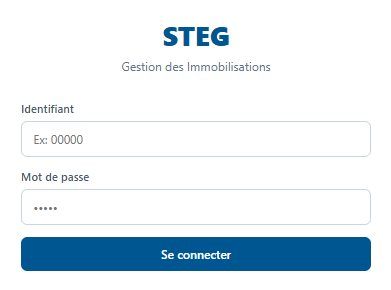
\includegraphics[width=0.9\textwidth]{../../assets/Authentification.png}
  \caption{Interface d'authentification}
  \label{fig:login_page}
\end{figure}

\subsection{Tableau de Bord Principal et Modules Associés}

Une fois l'authentification validée, le système affiche un tableau de bord centralisé qui offre une vue d'ensemble sur l'état du patrimoine. Cette page présente des indicateurs de synthèse sur le volume des immobilisations, la répartition des véhicules et les alertes d'inventaire en cours. Depuis ce tableau de bord, l'utilisateur accède aux différents modules fonctionnels de l'application.

\begin{figure}[H]
  \centering
  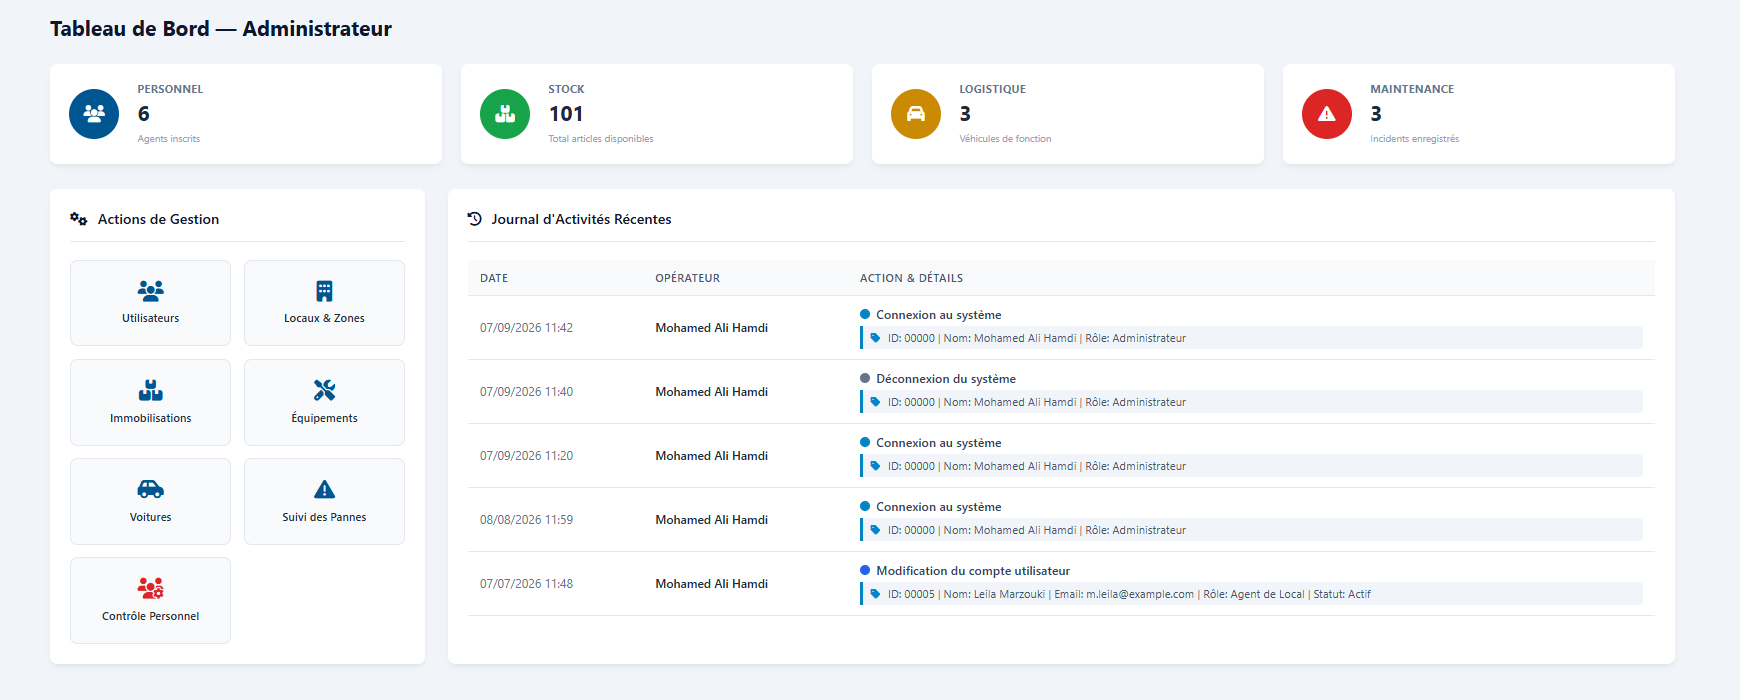
\includegraphics[width=0.9\textwidth]{../../assets/Dashboard.png}
  \caption{Tableau de bord de l'application}
  \label{fig:dashboard}
\end{figure}

\subsection{Module de Gestion des Utilisateurs}

\paragraph{Liste des Personnels}
Cette vue présente l'annuaire complet des agents enregistrés dans le système. Elle permet de visualiser rapidement les informations de contact, le département d'affectation ainsi que le rôle attribué à chaque utilisateur au sein de la plateforme.

\begin{figure}[H]
  \centering
  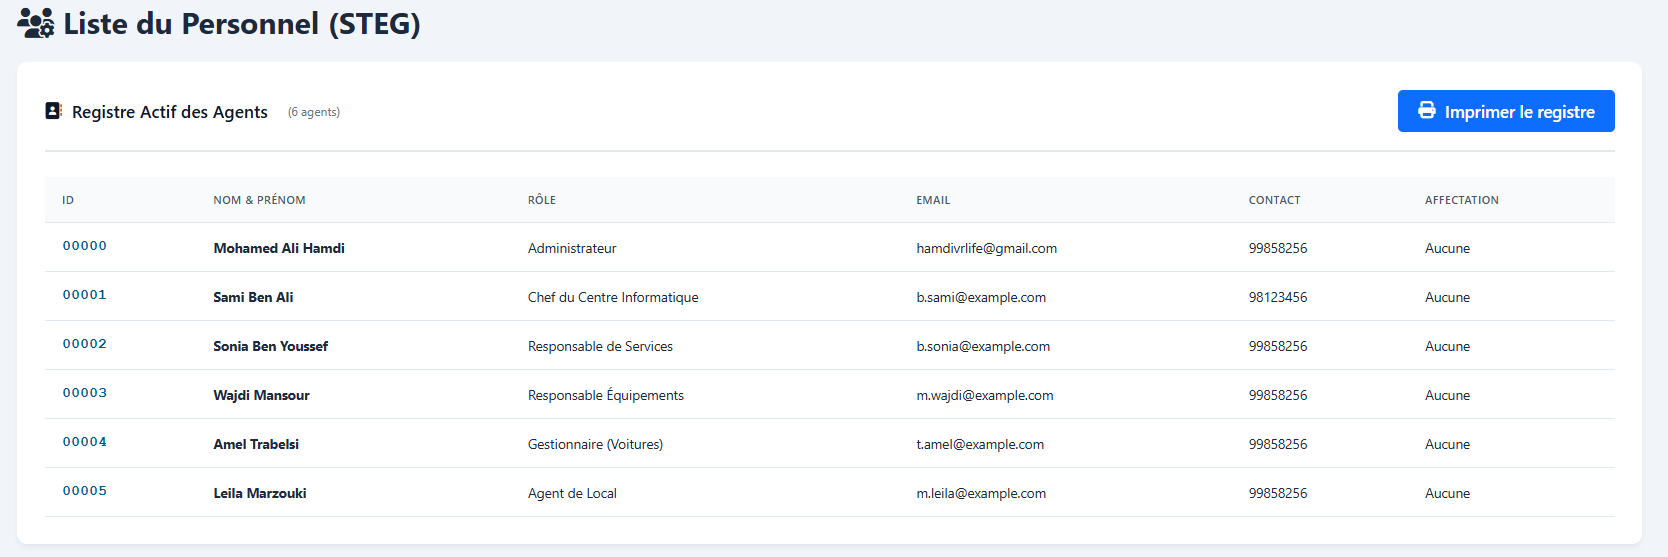
\includegraphics[width=0.9\textwidth]{../../assets/list_utilisateurs.png}
  \caption{Interface d'affichage de la liste des personnels}
  \label{fig:list_utilisateurs}
\end{figure}

\paragraph{Gestion des Personnels}
Cette interface administrative est dédiée à la création, à la modification et à la suppression des comptes utilisateurs. Elle permet également d'assigner les différents privilèges d'accès pour sécuriser les actions réalisables selon chaque profil.

\begin{figure}[H]
  \centering
  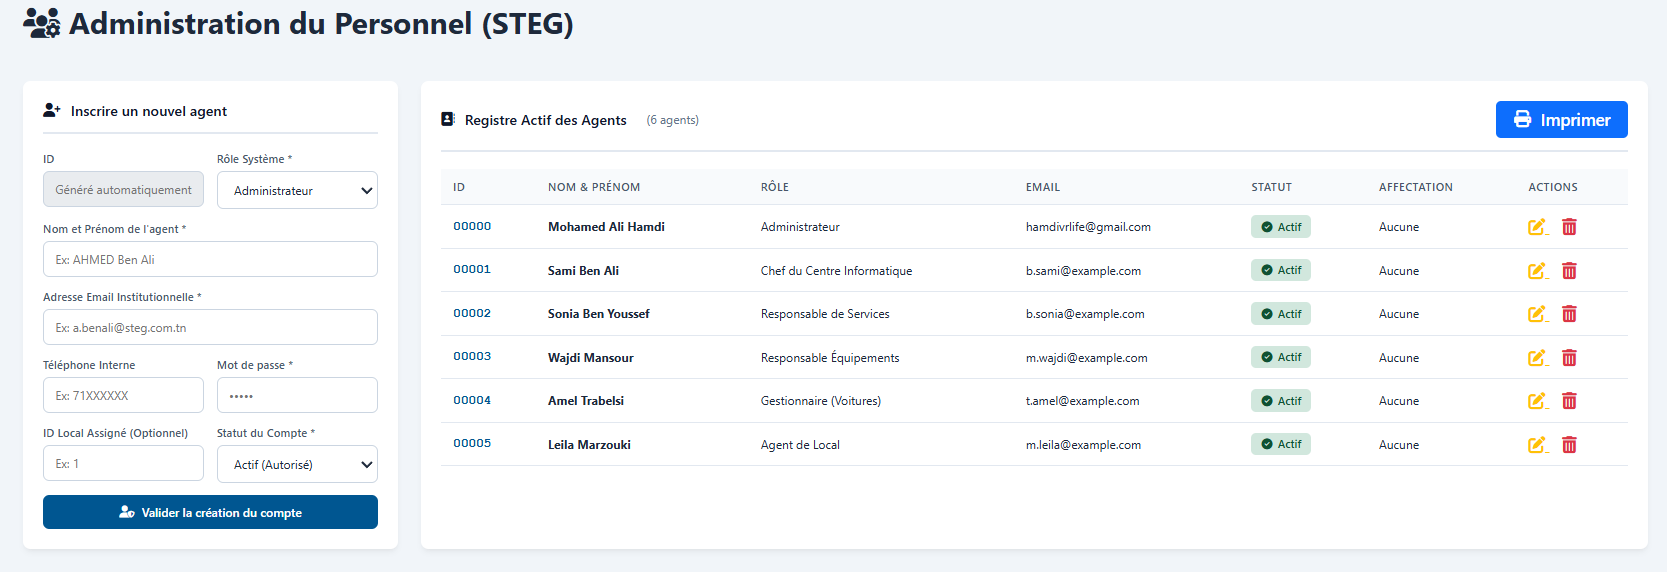
\includegraphics[width=0.9\textwidth]{../../assets/gestion_utilisateurs.png}
  \caption{Interface de gestion et d'administration des personnels}
  \label{fig:gestion_utilisateurs}
\end{figure}

\subsection{Module de Gestion des Locaux}

Ce module permet de structurer et d'administrer l'arborescence des différents bâtiments et salles de la structure. Il facilite le rattachement géographique des équipements et du personnel, garantissant ainsi une traçabilité spatiale rigoureuse de l'ensemble du patrimoine immobilier.

\begin{figure}[H]
  \centering
  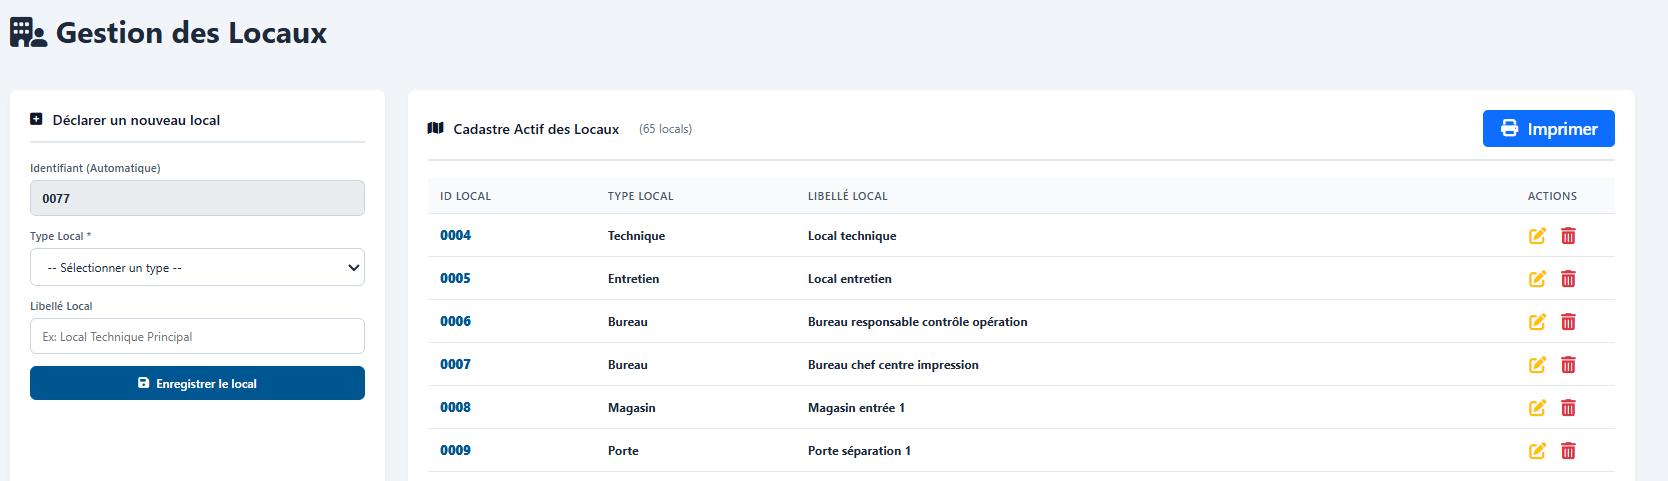
\includegraphics[width=0.9\textwidth]{../../assets/gestion_locaux.png}
  \caption{Interface de gestion des locaux}
  \label{fig:gestion_locaux}
\end{figure}

\subsection{Module de Gestion des Immobilisations}

Véritable cœur de l'application, ce module centralise l'inventaire général des biens de l'entreprise. Il permet l'enregistrement, la mise à jour et le suivi des fiches d'immobilisation, facilitant ainsi la gestion des acquisitions et la valorisation globale du patrimoine.

\begin{figure}[H]
  \centering
  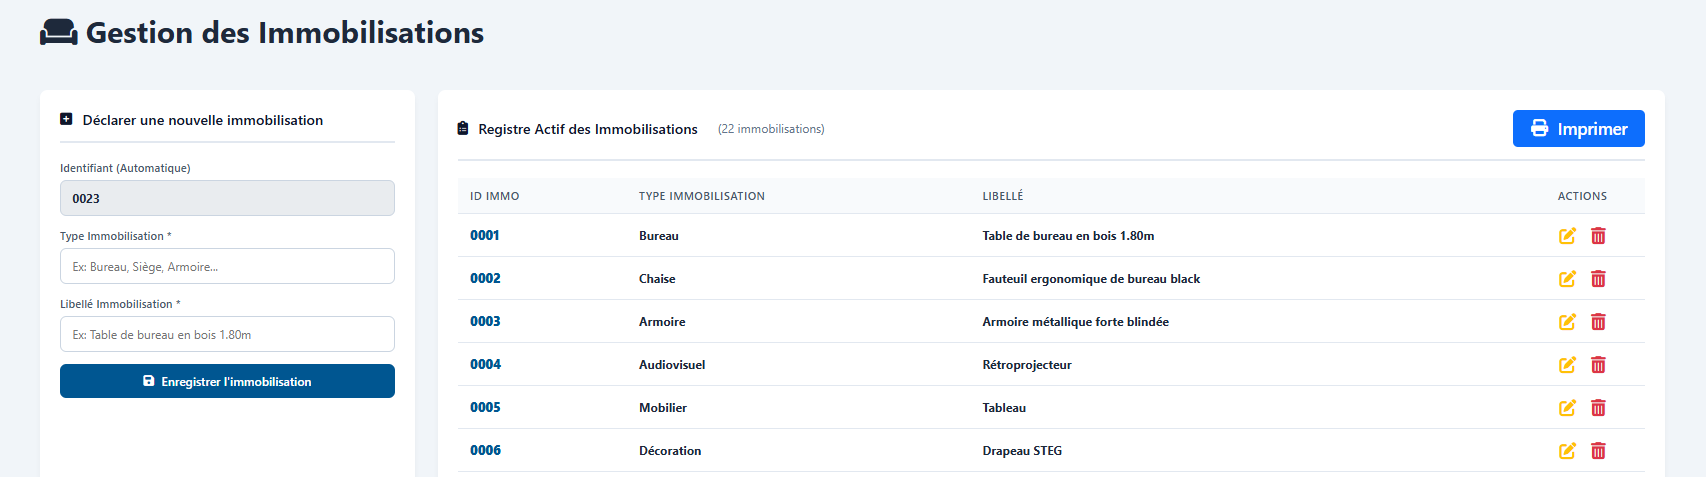
\includegraphics[width=0.9\textwidth]{../../assets/gestion_immobilisations.png}
  \caption{Interface de gestion des immobilisations}
  \label{fig:gestion_immobilisations}
\end{figure}

\subsection{Module de Suivi des Équipements}

Dédiée à la traçabilité des équipements techniques, cette vue permet d'enregistrer les équipements et de modifier leur état opérationnel, tout en conservant un historique fiable des mouvements.

\begin{figure}[H]
  \centering
  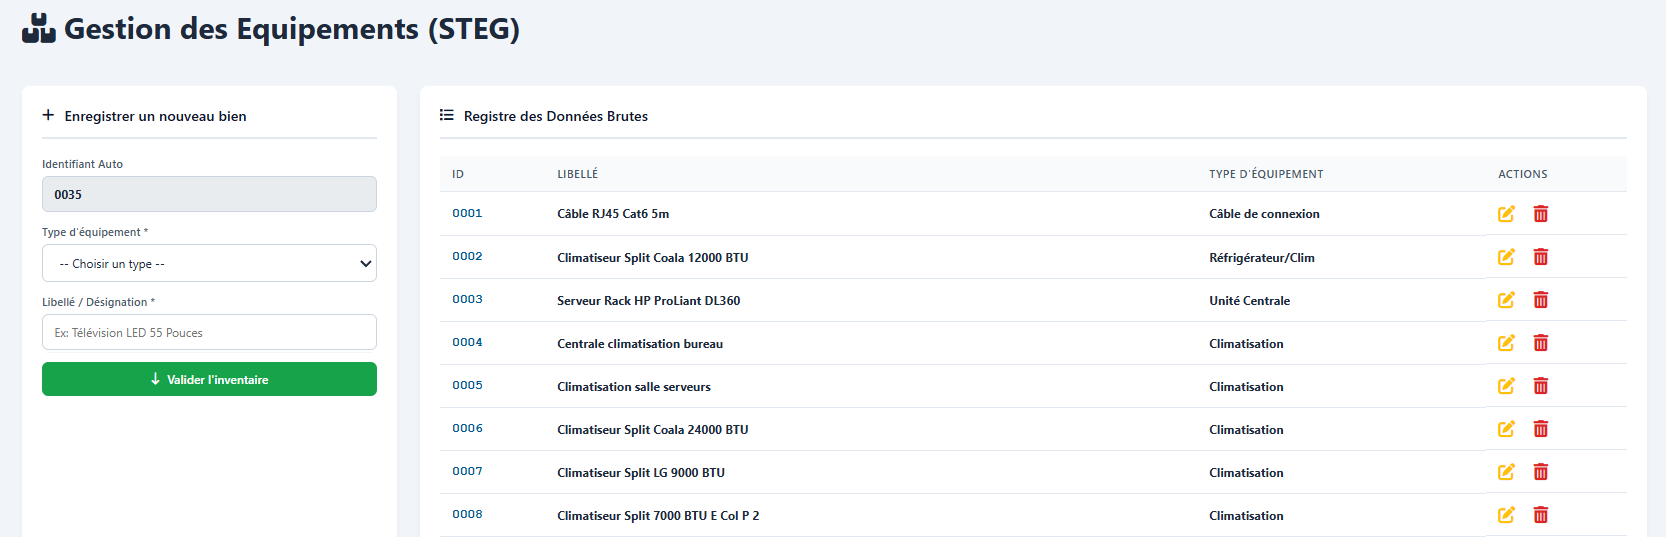
\includegraphics[width=0.9\textwidth]{../../assets/gestion_equipements.png}
  \caption{Interface de gestion des équipements}
  \label{fig:gestion_equipements}
\end{figure}

\subsection{Module de Gestion du Parc Automobile}

Cette section de l'application centralise l'ensemble des informations relatives à la flotte de véhicules de la société. Il permet le suivi des fiches techniques des voitures, de leur état général ainsi que de leurs directions d'affectation respectives.

\begin{figure}[H]
  \centering
  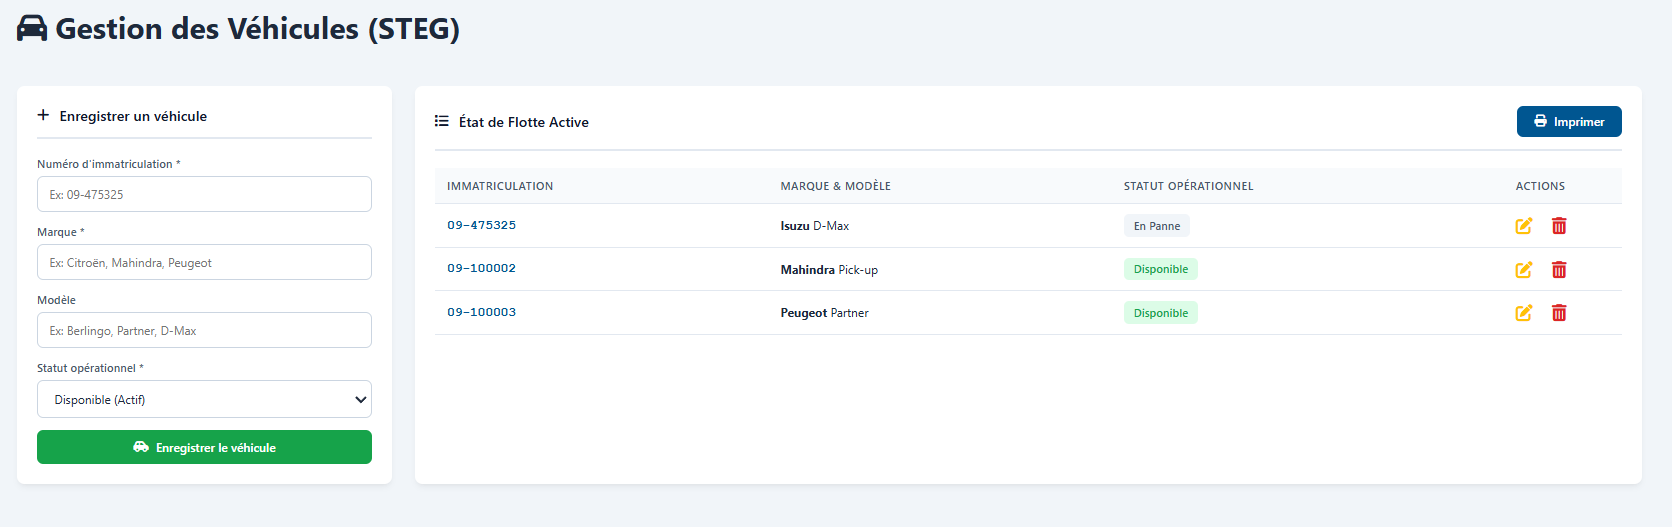
\includegraphics[width=0.9\textwidth]{../../assets/gestion_vehicules.png}
  \caption{Interface de suivi du parc roulant}
  \label{fig:gestion_vehicules}
\end{figure}

\subsection{Module de Gestion des Pannes}

Ce module est indispensable pour le suivi des dysfonctionnements signalés sur le matériel et les véhicules. Il permet de déclarer une nouvelle panne, d'attribuer un niveau de priorité, d'assurer le suivi des interventions de maintenance et de clôturer les tickets une fois la réparation effectuée.

\begin{figure}[H]
  \centering
  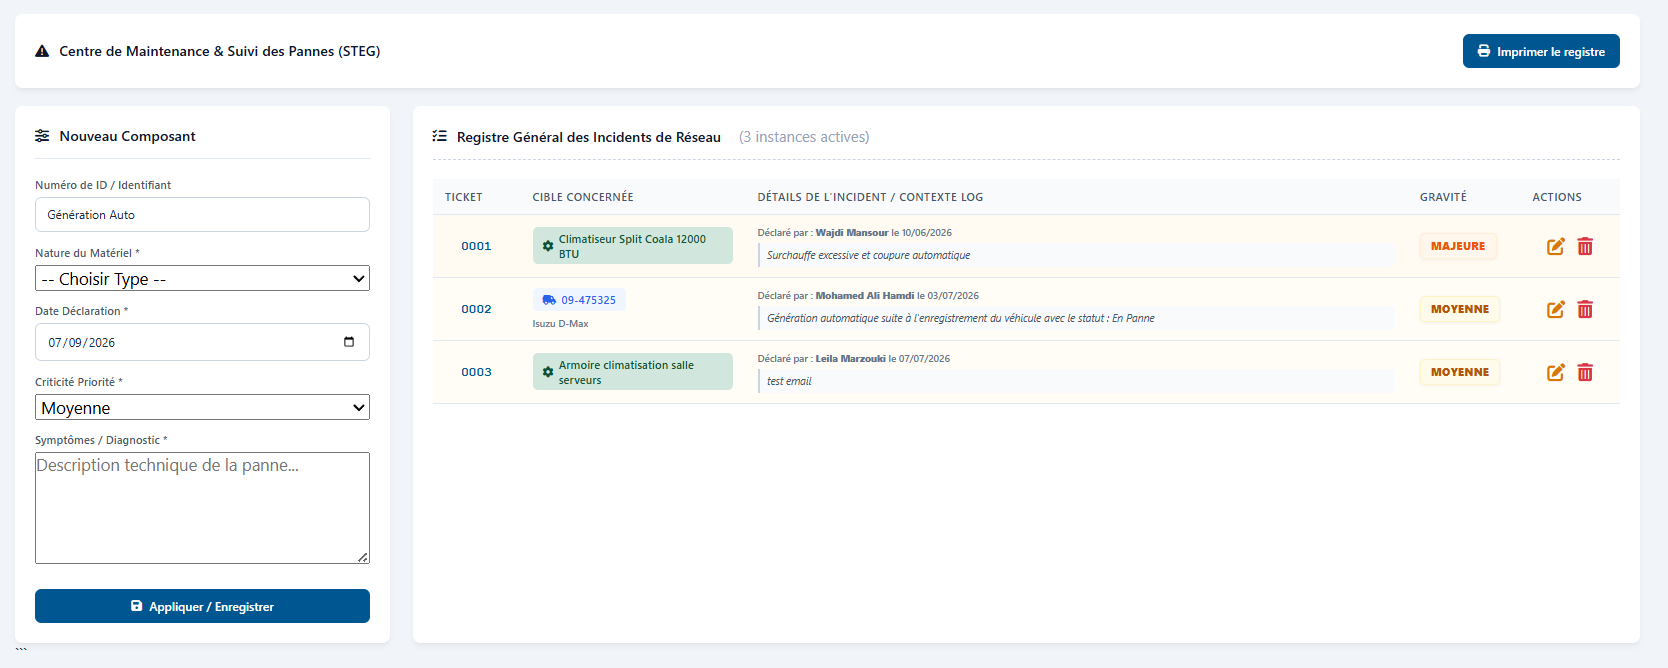
\includegraphics[width=0.9\textwidth]{../../assets/gestion_pannes.png}
  \caption{Interface de suivi des pannes}
  \label{fig:gestion_pannes}
\end{figure}

\subsection{Module de Gestion du Magasin}

Ce module gère les stocks de pièces de rechange et de matériel disponible en réserve. Il permet d'assurer un suivi rigoureux des entrées, des sorties et des seuils d'alerte des articles stockés.

\begin{figure}[H]
  \centering
  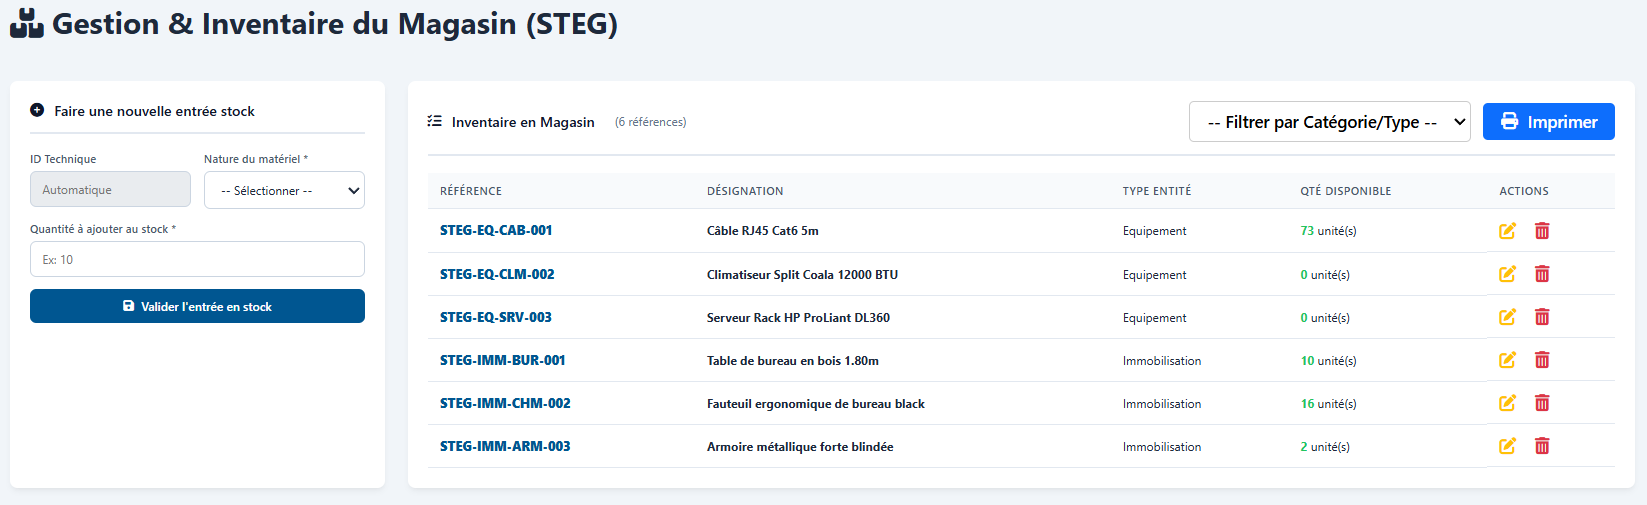
\includegraphics[width=0.9\textwidth]{../../assets/gestion_magasin.png}
  \caption{Interface de suivi du magasin}
  \label{fig:gestion_magasin}
\end{figure}

\subsection{Module de Gestion du Plan}

Cette section permet d'intégrer et de visualiser les plans architecturaux de la structure. Elle facilite la localisation interactive des immobilisations et des équipements directement sur les schémas des différents étages ou bâtiments.

\begin{figure}[H]
  \centering
  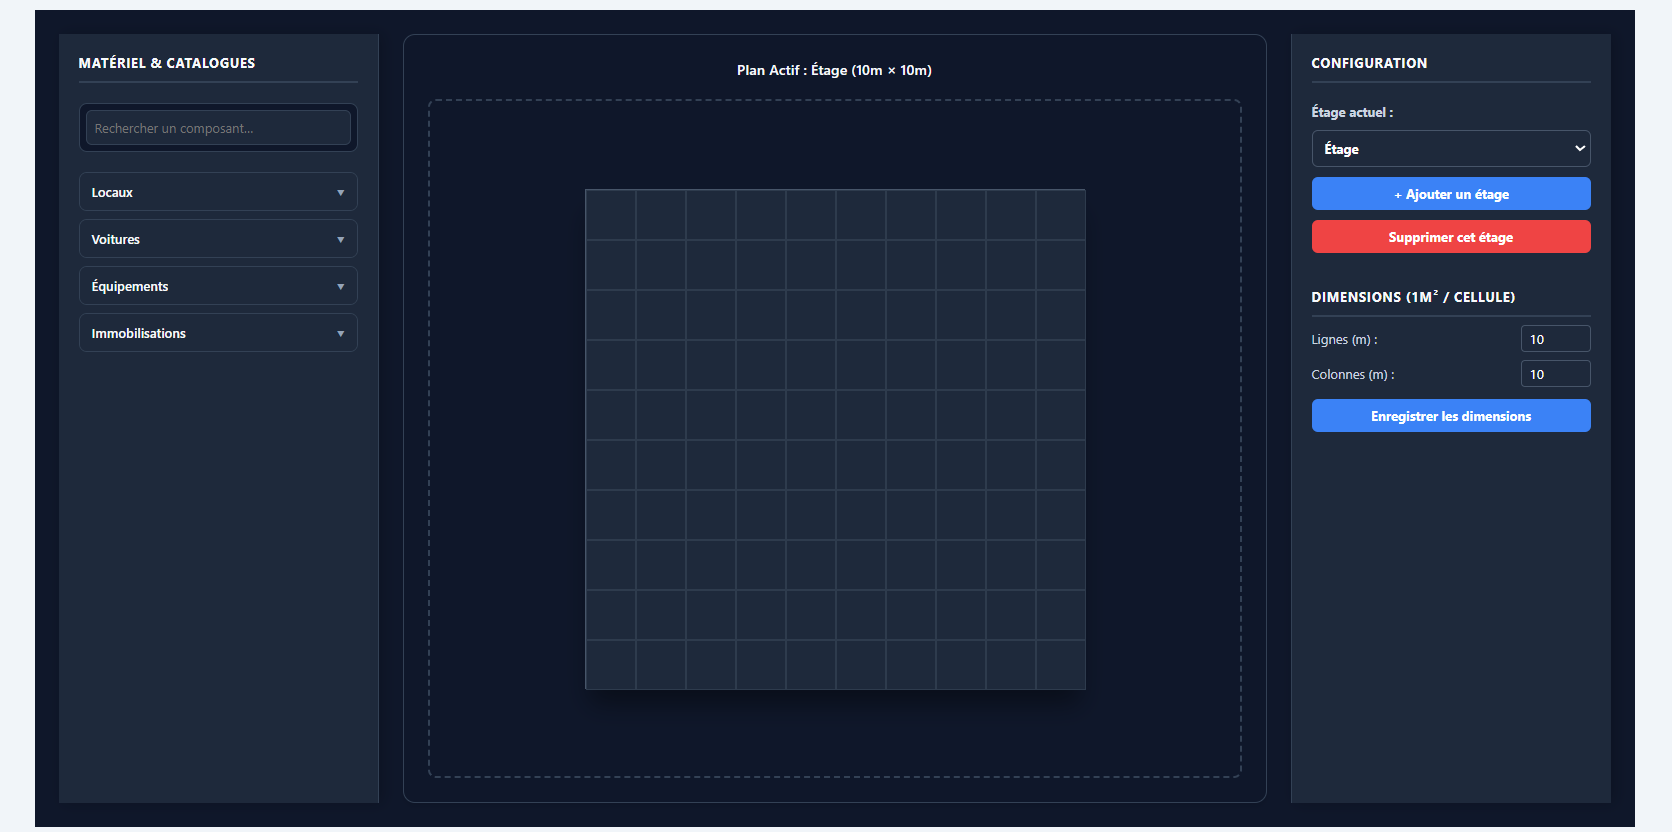
\includegraphics[width=0.9\textwidth]{../../assets/gestion_plan.png}
  \caption{Interface de suivi du plan}
  \label{fig:gestion_plan}
\end{figure}

\subsection{Module de Documentation}

Ce module centralise les guides d'utilisation, les manuels techniques et les historiques d'activité liés au système. Il permet de consulter ou de télécharger rapidement les ressources et journaux nécessaires à la bonne administration de la plateforme.

\begin{figure}[H]
  \centering
  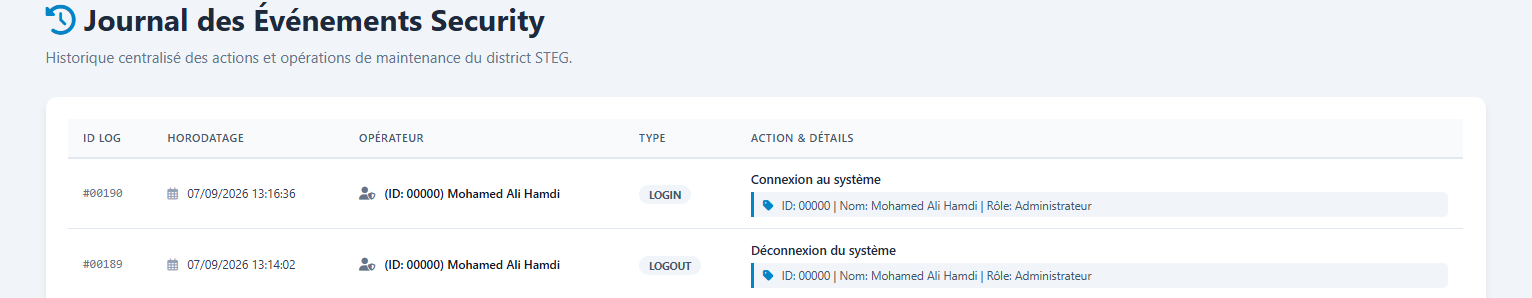
\includegraphics[width=0.9\textwidth]{../../assets/logs.png}
  \caption{Interface de gestion de la documentation}
  \label{fig:logs}
\end{figure}

\section{Conclusion du Chapitre}

En somme, cette phase de réalisation a permis de concrétiser l'ensemble des choix architecturaux et fonctionnels retenus lors de la conception. À travers le développement des différents modules, l'application offre désormais une solution opérationnelle, ergonomique et sécurisée pour la gestion globale du patrimoine. Le prochain chapitre sera consacré aux tests finaux et à la validation générale du projet.